\documentclass[doc, floatsintext]{apa7}
\usepackage[style=apa,sortcites=true,sorting=nyt,backend=biber]{biblatex}
\DeclareLanguageMapping{american}{american-apa}
\addbibresource{sample.bib}
\setlength\bibhang{.15in}
\usepackage{amsmath}
\usepackage{float}
\usepackage{graphicx}
\usepackage{mathrsfs}
\usepackage{setspace}
\setstretch{1.0}
\usepackage{caption}
\usepackage{gensymb}

\title{Criterial Learning and Feedback Delay: Insights from
Computational Models and Behavioral Experiments}
\shorttitle{Computational Criterion Learning}

\authorsnames[{1, 2}, {3}, {4}]{
    Matthew J. Crossley, 
    Benjamin O. Pelzer,
    F. Gregory Ashby
}

\authorsaffiliations{
    {School of Psychological Sciences, Macquarie University, Sydney, Australia}, 
    {Macquarie University Performance and Expertise Research Centre, Macquarie University, Sydney, Australia},
    {Independent Researcher},
    {Department of Psychological \& Brain Sciences, University of California, Santa Barbara}
    }

\abstract{
    The notion of a response criterion is ubiquitous in
    psychology, yet its cognitive and neural underpinnings
    remain poorly understood. To address this shortcoming,
    three computational models that capture different
    hypotheses about criterial learning were developed and
    tested. The time-dependent drift model assumes the
    criterion is stored in working memory and that its value
    drifts over time. The delay-sensitive learning model
    assumes that the magnitude of criterial learning is
    temporally discounted by feedback delay. The
    reinforcement-learning model assumes that criterial
    learning emerges from stimulus-response association
    learning without an explicit representation of the
    criterion, with learning rate also temporally discounted
    by feedback delay. The performance of these models was
    investigated under varying feedback delay and intertrial
    interval (ITI) durations. The time-dependent drift model
    predicted that long ITIs and feedback delays both impair
    criterial learning. In contrast, the delay-sensitive and
    reinforcement-learning models predicted impairments only
    with feedback delays.  Two behavioral experiments tested
    these predictions. In Experiment 1, participants were
    explicitly instructed about the relevant dimension to
    isolate criterial learning, and short feedback delays
    impaired learning relative to immediate feedback. In
    Experiment 2, using binary-feature stimuli without
    instruction (isolating rule selection/switching),
    neither longer ITIs nor delayed feedback affected
    performance. These results support the delay-sensitive
    and reinforcement-learning models, and suggest that even
    in tasks that appear to rely on explicit, rule-based
    reasoning, criterial learning may have strong
    associative underpinnings.
}

\authornote{Correspondence: Matthew J. Crossley, PhD,
  School of Psychological Sciences, Macquarie University,
  Australian Hearing Hub, 16 University Ave, Macquarie
  University, NSW 2109, Australia. Email:
  matthew.crossley@mq.edu.au 
}

\keywords{response criterion; criterial learning; associative learning; categorization; procedural learning}

\begin{document}
\maketitle 

\section{Introduction}
The notion of a response criterion is ubiquitous in
psychology. It is a key component of almost all decision
models. For example, the hypothesis that even YES-NO
detection decisions are determined by comparing the sensory
magnitude to a response criterion that is under the
observer's control, rather than to a fixed absolute
threshold, allowed signal detection theory to supplant
classical threshold theory as the dominant model in
psychophysics \parencite{GreenSwets1966}. All models that
include a response criterion assume its value is learned and
can shift if changes are made to instructions or payoffs. So
criterial learning is a fundamental component of almost all
decision-making models. Despite its importance, however, the
cognitive and neural mechanisms that underlie criterial
learning remain poorly understood.

This article addresses this shortcoming through a
combination of computational modeling and empirical data
collection. Specifically, we develop and test three
different computational models that make qualitatively
different assumptions about how the criterion is learned.
The models differ in the role they assign to working memory
and in whether they treat the response criterion as a
fundamental psychological construct, or instead assume that
behavior is driven purely by stimulus-response associations
without any criterion guiding responses. These models are
then tested in two behavioral experiments. The modeling and
empirical focus are on how feedback delays and the length of
the intertrial interval (ITI) affect criterial learning. All
criterial-learning models assume that updating (i.e.,
learning) of the criterion occurs during the time interval
between feedback presentation and the stimulus presentation
that defines the onset of the next trial. So feedback delay
and the length of the ITI are the independent variables that
most clearly differentiate the conflicting predictions of
criterial-learning models. Furthermore, feedback delays are
known to impair some forms of learning (i.e., procedural)
much more than others (i.e., learning that relies on
declarative memory), so feedback-delay manipulations offer a
powerful method of disambiguating the nature of criterial
learning \parencite{ell2009critrial, MaddoxAshbyBohil2003,
MaddoxIng2005}.

Although the models could be tested in any task that depends
on criterial learning, the two experiments we describe used
a one-dimensional category-learning task. In such tasks,
stimuli vary across trials on two or more dimensions -- one
relevant to categorization and one or more that are
irrelevant. The observer's goal is to identify the relevant
dimension and learn the response criterion that maximizes
accuracy. This task has been used in hundreds of studies,
and all current models of performance in this task emphasize
the role of criterial learning.

In the first behavioral experiment, participants were
explicitly instructed about the relevant dimension, thereby
isolating criterial learning from rule selection and
switching processes. The results showed that short feedback
delays impaired learning compared to immediate feedback.
The second behavioural experiment used stimuli composed of
binary features -- where no criterial learning is needed --
and did not instruct participants about the relevant
dimension. Thus, this experiment isolated rule selection and
switching from criterial learning. The results found that
increasing feedback delay or ITI did not affect performance.
These findings suggest that feedback delays impact criterial
learning but not the discovery of the relevant stimulus
dimension.  More broadly, they indicate that criterial
learning may recruit procedural learning, even in tasks that
seem to rely on explicit, rule-based processes.

\section{New Computational Models of Criterial Learning}
We developed computational models of criterial learning
within two broad architectures and examined their
sensitivity to ITI duration and feedback delay. The
architectures differ in whether they assume that the
response criterion is explicitly represented in memory. In
the first architecture, the criterion is stored in memory,
and responses are generated by comparing the current percept
with this stored referent. The criterion is updated after
errors using a gradient-descent rule. Models in this class
can exhibit sensitivity to ITI and feedback delay in three
distinct ways: (1) perceptual drift, where stimulus
representations change over time, (2) criterial drift, where
the stored criterion shifts over time, and (3)
delay-sensitive updating, where the magnitude of criterion
updates decreases with longer feedback delays. In the second
architecture, no explicit criterion is stored.  Instead,
reinforcement learning forms direct stimulus--response
associations that drive performance.  Sensitivity to ITI and
feedback delay arises from either perceptual drift or
delay-sensitive updating, but criterial drift is not
possible since no criterion is represented.

For each of these models, denote the time of stimulus
presentation on the current trial by T$_\text{S}$, the
response time by T$_\text{R}$, the time when feedback is
displayed by T$_\text{F}$, and the time when the stimulus
that begins the next trial is displayed by T$_{\text{S}^+}$.
Then note that the feedback delay equals $\text{t}_\text{FD}
= \text{T}_\text{F} - \text{T}_\text{R}$ and the duration of
the ITI equals $\text{t}_\text{ITI} = \text{T}_{\text{S}^+}
- \text{T}_\text{F}$.

\subsection{Models that assume a stored criterion}
These models assume that the observer constructs a response
criterion, maintains it in working memory, and makes
decisions by comparing the percept to this criterion. They
may further posit that both the stored criterion and the
perceived stimulus value drift over time, with the extent of
drift increasing both within a trial and across consecutive
trials. In addition, they may assume that the learning rate
for updating the criterion decreases as the feedback delay
increases.

Let $x_n(t)$ and $c_n(t)$ denote the values of the percept
and the criterion, respectively, on trial $n$ at time $t$.
Then the decision rule on trial $n$ is:
\begin{equation}
  \text{Respond } R_n =
  \begin{cases}
    \text{A}, & \text{if ~} x_n(\text{T}_\text{S}) \leq c_n(\text{T}_\text{S})  \\
    \text{B}, & \text{if ~} x_n(\text{T}_\text{S}) > c_n(\text{T}_\text{S}).
  \end{cases}
  \label{eq:DR}
\end{equation}
Note that this equation indicates that the response is made
immediately upon stimulus presentation. We therefore are not
explicitly modelling the time-extended cognitive processes
that govern evidence accumulation and the corresponding
response time.

If positive feedback is received, then the value of the
criterion remains unchanged for the next trial (except for
drift -- see Equation \ref{eq:criterion}).  The rationale
here is that if the response is correct, then the observer
has effectively gained zero information about how their
criterion should be modified.  If negative feedback is
received, then the criterion is modified according to the
standard model
\parencite{SuttonBarto1998}:
\begin{equation}
c_n(\text{T}_\text{F}+ \Delta_t) = c_n(\text{T}_\text{F}) + \frac{\alpha}{t_{FD}} [x_n(\text{T}_\text{F}) - c_n(\text{T}_\text{F})],
\label{RL}
\end{equation}
where $\alpha$ is a learning-rate parameter, and $\Delta_t$
is the time it takes to complete the updating.  It is
straightforward to show that the iterative Equation \ref{RL}
is equivalent to computing a weighted mean (weighted by
recency) of the values of all percepts that occur on error
trials \parencite[e.g.,][]{Ashby2017}. This updating rule
will gradually converge on the optimal criterion value
(i.e., the true criterion value the observer is trying to
learn).  

The term $\frac{\alpha}{t_{FD}}$ captures the notion that
the magnitude of the update decreases as the feedback delay
increases.  As a result, when feedback is delayed, the
system becomes less responsive to errors, leading to slower
learning compared to immediate feedback conditions. However,
since this model is consistent with the idea that criterial
learning relies on working memory -- and the available
evidence suggests that logical reasoning and working memory
are unaffected by feedback delays of several seconds
\parencite[e.g., in one-dimensional rule-based category
learning tasks;][]{ell2009critrial, MaddoxAshbyBohil2003,
MaddoxIng2005} -- the learning process described in Equation
\ref{RL} likewise be unaffected by feedback delay. In this
case, the term $\frac{\alpha}{t_{FD}}$ is replaced by
$\alpha$, making the learning rate independent of feedback
delay.

This model further assumes that both the stimulus and the
criterion representations may drift randomly throughout the
duration of time they are maintained in working memory. The
representation of the criterion must always be maintained in
working memory, whereas drift in the stimulus representation
affects performance up until the feedback is presented, but
not afterwards. We modeled the drift in both the criterion
and the percept by adding white noise to their initial
values. Specifically, we assumed that for all
$t>\text{T}_\text{S}$
\begin{equation}
  c_n(t) = c_n(\text{T}_\text{S}) + \eta_c \epsilon(t),
  \label{eq:criterion}
\end{equation}
and
\begin{equation}
  x_n(t) = x_n(\text{T}_\text{S}) + \eta_x \epsilon(t),
  \label{eq:percept}
\end{equation}
where $\epsilon(t)$ is white noise and $\eta_c$ and $\eta_x$
are parameters that determine the amount of drift over time.
Note that these parameters are permitted to be equal to zero
which is equivalent to assuming that the criterion and/or
the percept do not drift over time at all.

This model predicts that at the time of feedback, the
response criterion $c_n(\text{T}_\text{F})$ will be normally
distributed with mean $c_n(\text{T}_\text{S})$ and variance
$\text{t}_\text{FD} \eta_c^2$. Similarly, at the time when
the stimulus that defines the next trial is presented, the
criterion $c_n(\text{T}_{\text{S}^+}) =
c_{n+1}(\text{T}_\text{S})$ is normally distributed with
mean $c_n(\text{T}_\text{S})$ and variance
$(\text{t}_\text{FD}+\text{t}_\text{ITI}) \eta_c^2$. The
predictions for the percept are similar. Specifically, at
the time when feedback is presented, the percept
$x_n(\text{T}_\text{F})$ is normally distributed with mean
$x_n(\text{T}_\text{S})$ and variance
$(\text{T}_\text{F}-\text{T}_\text{S}) \eta_x^2$.

\subsection{Reinforcement-learning models}
The reinforcement-learning models gradually associate
responses with stimuli, and therefore do not include an
explicit representation of the response criterion. The
models are based on an actor-critic architecture and use
reinforcement learning to form stimulus-response
associations \parencite{SuttonBarto1998}. These models
assumes that the perceptual representation of each stimulus
is defined by the pattern of activation across 25 sensory
units that are characterized by overlapping tuning curves.
Each unit is maximally excited by one specific stimulus,
which we call the unit's preferred stimulus. Specifically,
the activation of the $i^\text{th}$ sensory unit on trial
$n$ is given by
\begin{equation}
  A_i(n) = \text{exp} \left( \frac{-\left[d_{i,S_n}\right]^2}{\sigma^2} \right)
  \label{eq:DSL_activation}
\end{equation}
where $d_{i,S_n}$ is the (Euclidean) distance between the preferred
stimulus value of the $i^\text{th}$ sensory unit and the
value of the stimulus that was presented on trial $n$, and
$\sigma$ is a constant that increases with perceptual noise.

The model includes two decision or actor units -- one
associated with each of the two possible responses.
Initially, each sensory unit is connected to both actor
units with some random connection strength. Let
$\omega_{iJ}(n)$ denote the strength of the connection
between sensory unit $i$ and actor unit $J$ (for $J$ = A or
B) on trial $n$. Then the activation in actor unit $J$ on
trial $n$, denoted by $V_J(n)$, equals
\begin{equation}
  V_J(n) = \sum_{i} \omega_{iJ}(n) A_i(n)
\end{equation}
Responses are generated by the decision rule:
\begin{equation}
 \text{Respond } R_n =
  \begin{cases}
    A, & \text{if $V_A(n) > V_B(n)$}\\
    B, & \text{if $V_A(n) \leq V_B(n).$}
  \end{cases}
\end{equation}
The connection strengths $\omega_{iA}(n)$ and
$\omega_{iB}(n)$ are updated after feedback is received on
each trial according to standard reinforcement learning
rules \parencite{SuttonBarto1998}:
\begin{equation}
  \omega_{iA}(n) = \omega_{iA}(n-1) + \frac{\alpha_{actor}}{t_\text{FD}} \delta(n-1)
\end{equation}
\begin{equation}
  \omega_{iB}(n) = \omega_{iB}(n-1) + \frac{\alpha_{actor}}{t_\text{FD}} \delta(n-1),
\end{equation}
where $\alpha_{actor}$ is the learning-rate of the actor, and
$\delta(n-1)$ is the reward prediction error on trial $n-1$.
Note that as in Equation~\ref{RL}, the learning rate is
scaled by the inverse of the feedback delay. 

Much evidence suggests that this type of stimulus-response
learning is mediated largely within the striatum, and is
facilitated by a dopamine (DA) mediated reinforcement
learning signal that is time dependent
\parencite[e.g.,][]{ValentinMaddoxAshby2014}. Specifically,
the dopamine signal generated by positive feedback appears
to peak at around 500 ms after feedback and then decay back
to baseline levels within 2 or 3 s
\parencite{YagishitaEtAl2014}. As a result, synaptic
plasticity at cortical-striatal synapses is attenuated with
increasing feedback delays \parencite{YagishitaEtAl2014}.
The scaling of $\alpha_{actor}$ by ${1}{t_\text{FD}}$ is one
way to model this phenomenon. However, it is possible that
criterial learning via stimulus-response associations is
mediated by other brain systems that are less sensitive to
feedback delay. In this case, the learning rate would be
independent of feedback delay, and the term
$\frac{\alpha_{actor}}{t_\text{FD}}$ would be replaced by
$\alpha_{actor}$.

The reward prediction error on trial $n-1$ is defined as the
value of the obtained reward, denoted by $R(n-1)$ minus the
value of the predicted reward, denoted by $P(n-1)$:
\begin{equation}
  \delta(n-1) = R(n-1) - P(n-1).
\end{equation}
The predicted reward on trial $n$ is determined by the
critic via
\begin{equation}
  P(n) = P(n-1) + \frac{\alpha_{critic}}{t_\text{FD}} \delta(n-1),
\end{equation}
where $\alpha_{critic}$ is the learning rate of the critic.
This learning rate may again be scaled by the inverse of the
feedback delay. If sensitivity to feedback delay is not
assumed in Equation~\ref{RL}, then the term
$\frac{\alpha_{critic}}{t_\text{FD}}$ is replaced by
$\alpha_{critic}$.

Because this class of models does not store an explicit
response criterion, it cannot incorporate criterial drift.
It can, however, incorporate perceptual drift. In this case,
the value of the current stimulus used to compute sensory
unit activation (Equation~\ref{eq:DSL_activation}) is
assumed to drift over time according to
\begin{equation}
  S_n(t) = S_n(\text{T}_\text{S}) + \eta_S \epsilon(t),
  \label{eq:stimulus_drift_RL}
\end{equation}
where $\eta_c$ scales the magnitude of the drift and
$\epsilon(t)$ is a noise process.

\subsection{Simulation Results}
We investigated how changing the duration of the feedback
delay and ITI affect criterial learning for each class of
model. More specifically, we simulated performance of
each model in a categorization task that included two
categories of stimuli that varied on a single stimulus
dimension and that could be categorized perfectly by
comparing each stimulus to an appropriate value of the
response criterion (We used the same experimental design as
in Experiment 1, so see those methods for more details). Our
simulations included three experimental conditions: Delayed
Feedback, Long ITI, and Control. The Delayed-Feedback
condition included a long feedback delay (3.5 s) and a short
ITI (0.5 s). The Long-ITI condition matched the total trial
duration of the Delayed-Feedback condition but with a short
feedback delay (0.5 s) and a long ITI (3.5 s). The Control
condition included both a short feedback delay (0.5 s) and a
short ITI (0.5 s). Each simulation continued for 200 trials
or until the model responded correctly for 12 trials in a
row. For each set of parameter values, we simulated the
model 100 times and averaged the results, yielding one
observed performance metric measured in trials-to-criterion
for each condition. 

Our approach was to generate predictions for each of the
three experimental conditions across a wide range of
parameter values. We then used parameter-space partitioning
(PSP) to evaluate the performance of each model
\parencite[PSP;][]{pitt2006global}.  Classical PSP is
defined for non-stochastic models and is often implemented
by exploring the parameter space via MCMC.  In contrast, we
used brute force search over a grid of plausible parameter
values. Because our models are stochastic, at each sampled
parameter setting we generated multiple simulations and
classified the expected qualitative pattern.  PSP calculates
the proportion of the parameter space where a model makes
specific qualitative predictions. We focused on four such
predictions. The first was that learning under feedback
delay would be slower than in the other two conditions. The
second was that learning in the Long ITI condition would be
slower than in the other two. The third was that learning in
the control condition would be slower than in either of the
other two conditions. The fourth was a catch-all category
encompassing any other possible patterns of results. For
each model, the PSP analysis quantified the proportions of
the explored parameter space where the model made these
qualitative predictions.

\subsubsection{Models that assume a stored criterion}
We investigated predictions of these models across a wide
range of values for the parameters $\eta_{x}$, $\eta_{c}$,
and $\alpha$.  Specifically, in the case of $\alpha$,  we
stepped through every value in the interval $[0, 0.2]$, with
a step size of .01.  In the case of both $\eta_{x}$, and
$\eta_{c}$, we searched over the interval $[0, 1]$, with a
step size of $0.1$.  We also explored the binary case of
whether or not the update rate $\alpha$ was scaled by the
feedback delay. The results are shown in Figure
\ref{fig:model_class_II_results}. 

\begin{figure} 
  \centering
  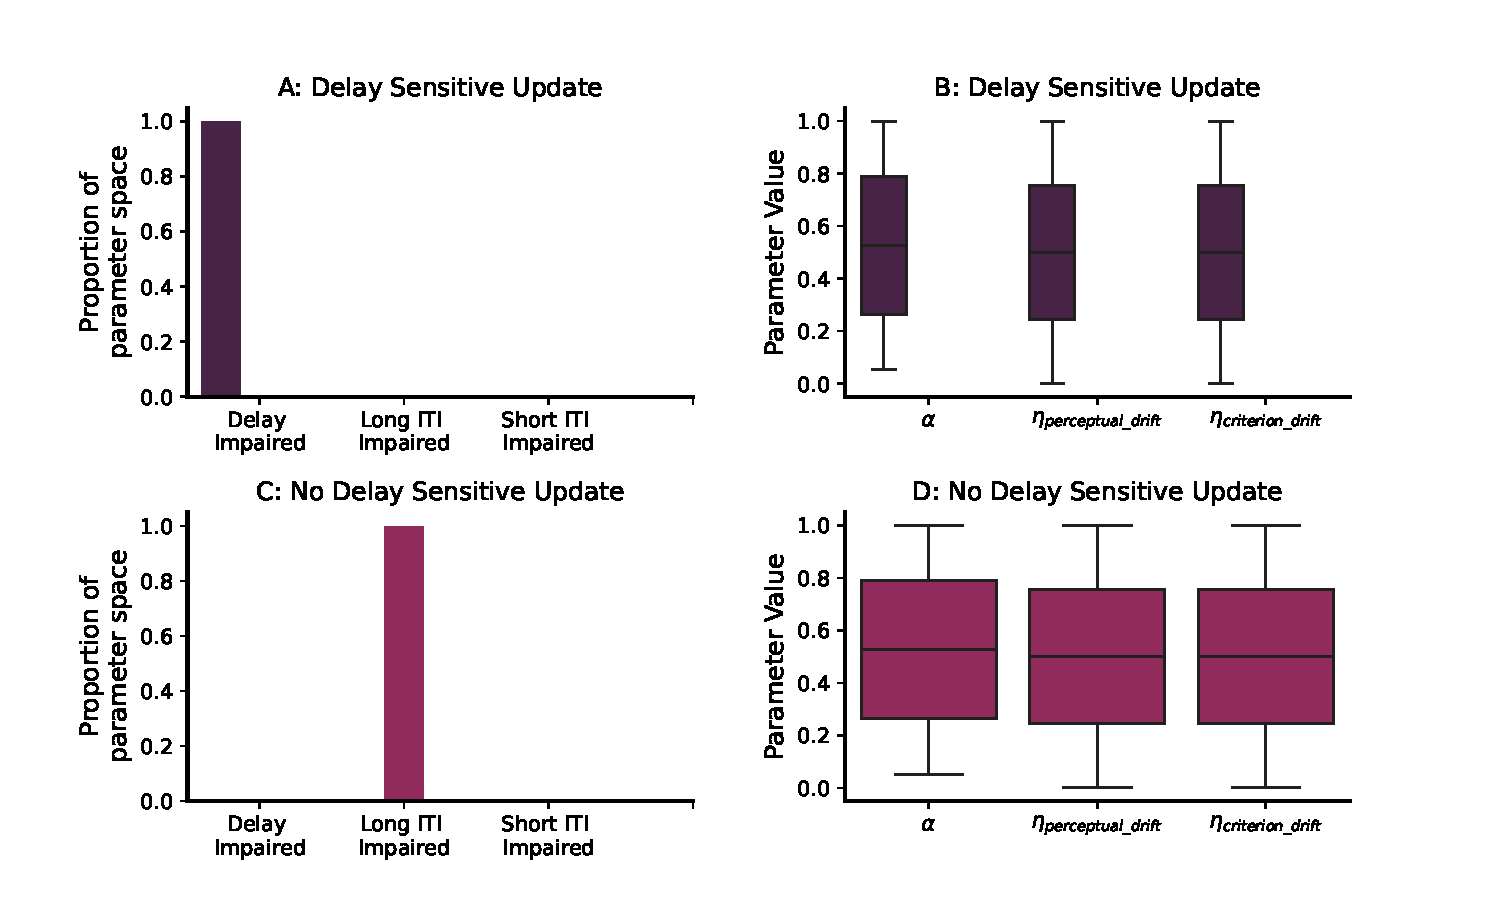
\includegraphics[width=1\textwidth]{../figures/model_new_class_II.pdf}
  \caption{ 
      \textbf{A:} Assuming a delay-sensitive update, the
      proportion of parameter space where the models that
      assume a stored criterion predicted each of four
      qualitative patterns: (1) slower learning under
      feedback delay, (2) slower learning in the Long-ITI
      condition, (3) slower learning in the control
      condition, and (4) any other pattern. 
      % 
      \textbf{B:} Assuming a delay-sensitive update, Boxplot
      of the parameter ranges leading to each PSP pattern.
      All parameter values were normalized by the largest
      value in the search range, so the ordinate ranges from
      zero to one for all parameters.
      % 
      \textbf{C:} Assuming no delay-sensitive update, the
      proportion of parameter space where the models that
      assume a stored criterion predicted each of four
      qualitative patterns: (1) slower learning under
      feedback delay, (2) slower learning in the Long-ITI
      condition, (3) slower learning in the control
      condition, and (4) any other pattern. 
      % 
      \textbf{D:} Assuming no delay-sensitive update, Boxplot
      of the parameter ranges leading to each PSP pattern.
      All parameter values were normalized by the largest
      value in the search range, so the ordinate ranges from
      zero to one for all parameters.
      %
      \textit{Note:} In all panels, color indicates the PSP
      pattern.
}
  \label{fig:model_class_II_results}
\end{figure}

Figure~\ref{fig:model_class_II_results} shows that this
class of models makes qualitatively different predictions
depending on whether the update rule is sensitive to
feedback delay. When delay sensitivity is assumed (panels A
and B), the model consistently predicts that feedback delays
impair criterion learning. When delay sensitivity is not
assumed (panels C and D), the model instead predicts that
long ITIs impair learning, except in cases with very small
learning rates $\alpha$ (panel D).

\subsubsection{Reinforcement-learning models}
We investigated the effects on performance predicted by the
reinforcement-learning model of three parameters -- the
perceptual-noise variance $\sigma^2$ and the actor and
critic learning rates (i.e., $\alpha_{actor}$ and
$\alpha_{critic}$, respectively). In the case of both
$\alpha_{actor}$ and $\alpha_{critic}$, we stepped through
every value in the interval $[0, 0.2]$, with a step size of
$.02$. We constrained our search over these parameters to this
interval because reinforcement-learning models are prone to
instability at very high learning rates
\parencite{SuttonBarto1998}. As evidence of this, at higher
learning rates, the model failed to learn with any
consistency -- that is, in most cases, it failed to reach
the learning criterion (12 correct responses in a row)
within the allowable 200 trials. In the case of $\sigma$, we
searched over the interval $[1, 10]$, with a step size of
$3$.  We also explored the binary case of whether or not the
update rate $\alpha$ was scaled by the feedback delay. As
with the other models, all scores were normalized by the
largest observed value.

The results are described in
Figure~\ref{fig:model_class_I_results}.  Note this model
predicts that delayed feedback impairs criterial learning
more than a long ITI across the vast majority of parameters
explored. As can be seen in
Figure~\ref{fig:model_class_I_results}D, the few exceptions
tend to occur when perceptual drift has relatively small
values.  

\begin{figure} 
  \centering
  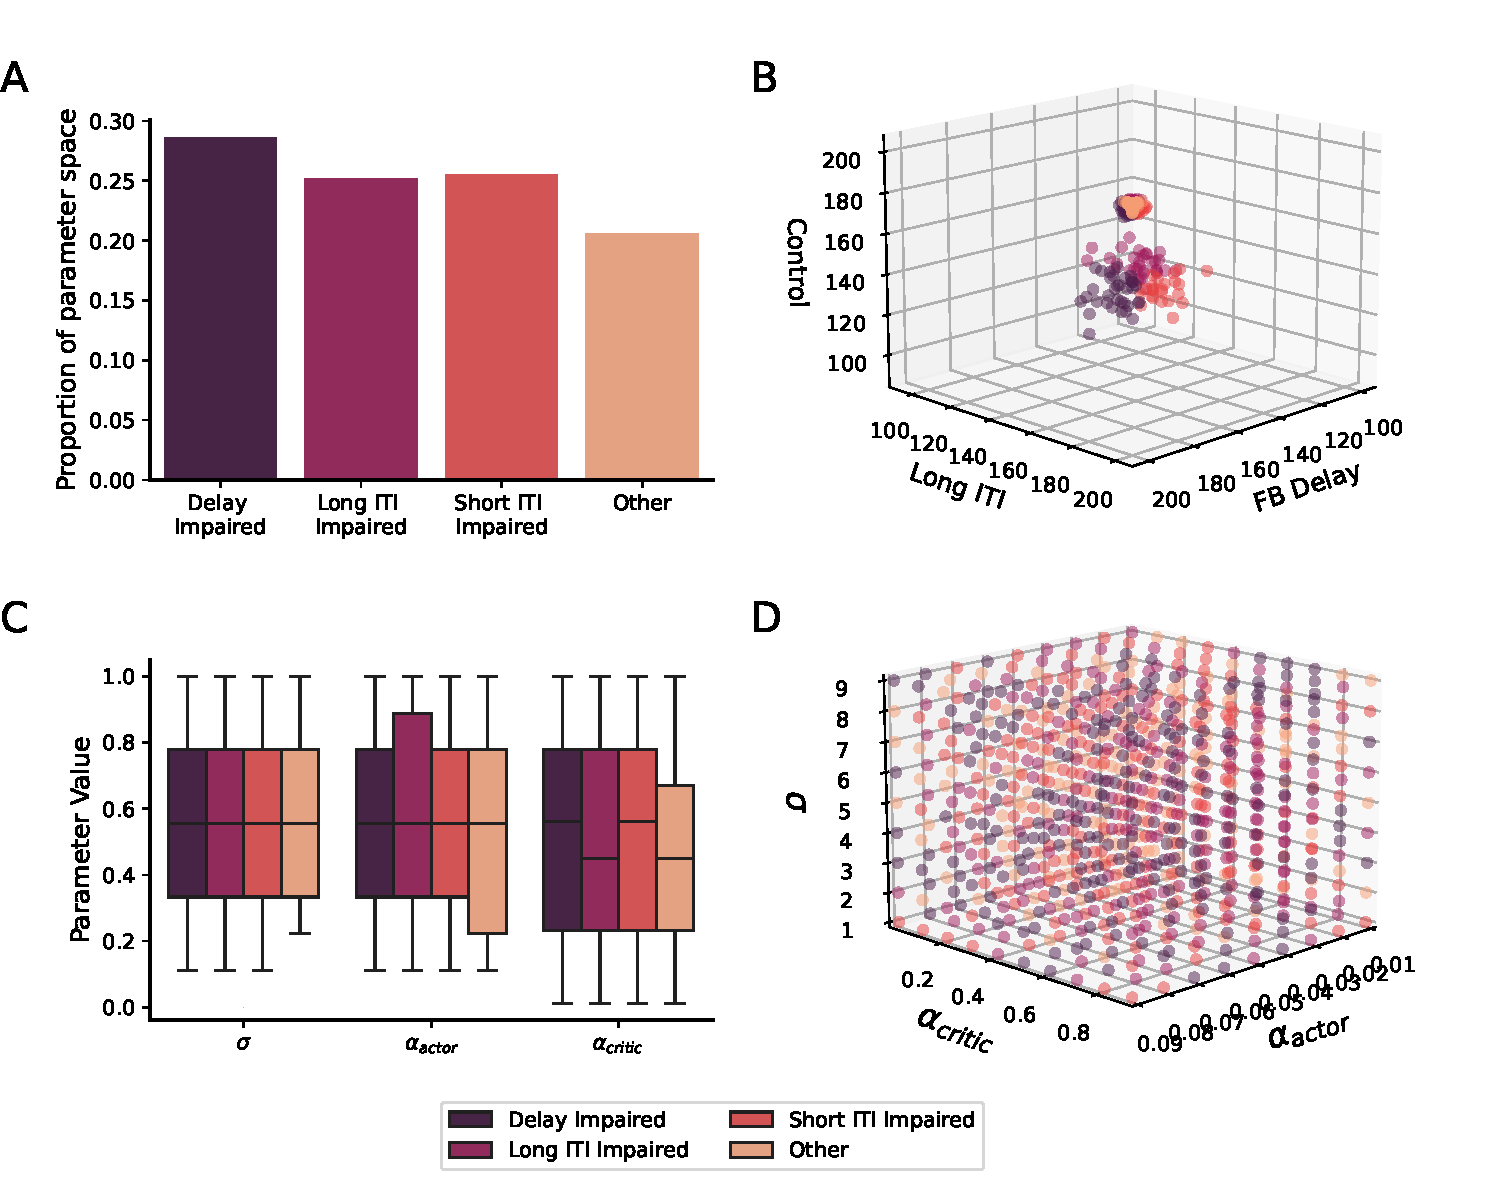
\includegraphics[width=1\textwidth]{../figures/model_new_class_I.pdf}
  \caption{ 
      \textbf{A:} Assuming a delay-sensitive update, the
      proportion of parameter space where the models that
      assume a stored criterion predicted each of four
      qualitative patterns: (1) slower learning under
      feedback delay, (2) slower learning in the Long-ITI
      condition, (3) slower learning in the control
      condition, and (4) any other pattern. 
      % 
      \textbf{B:} Assuming a delay-sensitive update, Boxplot
      of the parameter ranges leading to each PSP pattern.
      All parameter values were normalized by the largest
      value in the search range, so the ordinate ranges from
      zero to one for all parameters.
      % 
      \textbf{C:} Assuming no delay-sensitive update, the
      proportion of parameter space where the models that
      assume a stored criterion predicted each of four
      qualitative patterns: (1) slower learning under
      feedback delay, (2) slower learning in the Long-ITI
      condition, (3) slower learning in the control
      condition, and (4) any other pattern. 
      % 
      \textbf{D:} Assuming no delay-sensitive update, Boxplot
      of the parameter ranges leading to each PSP pattern.
      All parameter values were normalized by the largest
      value in the search range, so the ordinate ranges from
      zero to one for all parameters.
      %
      \textit{Note:} In all panels, color indicates the PSP
      pattern.
}
  \label{fig:model_class_I_results}
\end{figure}

\subsubsection{Summary of modeling results}
We examined two classes of criterial-learning models that
make different predictions about the effects of feedback
delay and ITI. The first class assumes that the criterion is
stored in memory and compared against incoming stimuli to
generate responses. These models predict greater impairment
from feedback delay only when the update rule is explicitly
delay-sensitive. Otherwise, they are generally more impaired
by long ITIs than by feedback delay. The second class
assumes no stored criterion, with responses driven instead
by reinforcement learning through gradual tuning of
stimulus–response associations. These models almost
uniformly predict greater impairment from feedback delay
than from long ITIs.

\section{Experiment 1}
Experiment 1 investigated how feedback delay and the length
of the ITI affect criterial learning in humans. As a result,
it also provides rigorous tests of the predictions of the
time-dependent drift model, the delay-sensitive learning
model, and the reinforcement-learning model.

The stimuli in Experiment 1 were circular sine-wave gratings
that varied across trials in bar width and bar orientation.
These stimuli were divided into two categories according to
their value on one of the two dimensions. In other words,
the optimal strategy was to set a response criterion on the
single relevant dimension, and then choose a categorization
response based on whether the value of the presented stimuli
on this dimension was larger or smaller than the criterion
value. 

The experiment isolated criterial learning by (1) explicitly
instructing participants on the relevant stimulus dimension
and rule structure (e.g., thick bars are ``A'', thin bars
are ``B''), and (2) eliminating variability along the
irrelevant stimulus dimension. In other words, the
instructions identified the relevant stimulus dimension, and
as a result, the only learning required was criterial
learning. 

\subsection{Method}

\subsubsection{Apparatus}
All experiments were performed in a dimly lit room.
Participants sat approximately 24'' from a 17'' $\times$
11'' monitor running at a resolution of 1680 $\times$ 1050
pixels. Participants made category judgments by pressing the
`d' or `k' keys on a standard computer keyboard for `A' or
`B' choices, respectively. Stickers with bold print `A' or
`B' were placed on the appropriate keys.

\subsubsection{Stimuli and Categories}
Stimuli were circular sine-wave gratings that varied in bar
width and bar orientation, drawn from various 1-dimensional
uniform distributions specific to the current category
problem. We first defined an arbitrary 2-dimensional
$[0-100,0-100]$ stimulus space, and then split each
dimension of this space into 7 bins of width 14 units each.
Each $(x,y)$ pair from this arbitrary stimulus space was
converted to a grating according to the nonlinear
transformations defined by
\textcite{treutwein1989perceptual}, which roughly equate the
salience of each dimension (for details, see also
\textcite{CrossleyAshby2015}).

The structure of the various criterial-learning tasks is
illustrated in Figure \ref{fig_design_exp_1_space}. Each
criterial-learning problem was created by first selecting a
relevant dimension. This was spatial frequency for the
problems 1 thorugh 7 and orientation for problems 8 through
14. We then randomly selected one of the 7 bins defined on
that dimension. Each bin was also associated with a
corresponding unique value on the irrelevant dimension. We
buffered the to-be-learned response criterion by 10\% of
total bin width on either side with a no-stimulus region.
Random uniform samples from the remaining eligible region of
each bin were then selected and presented to the participant
until 9 correct responses out of any 10 responses in a row
advanced the participant to the next problem. Note that
every category problem was a simple one-dimensional rule in
which optimal accuracy was 100\%.  Note also that the
relative location of the optimal response criterion varied
across problems.

\begin{figure}
  \centering
  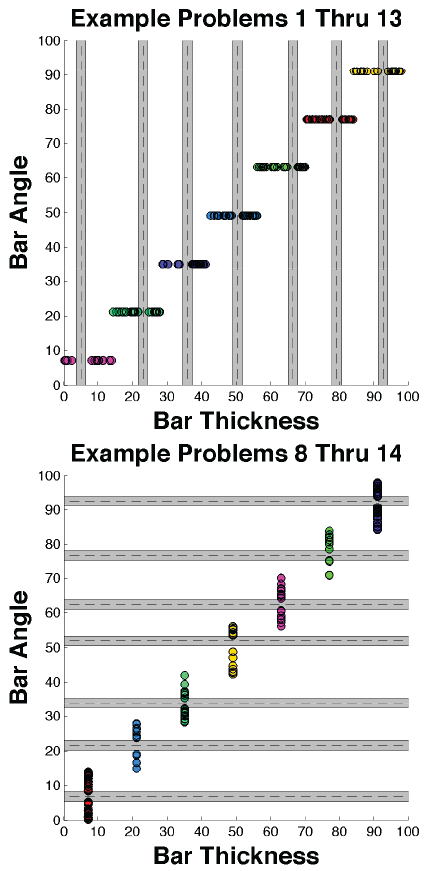
\includegraphics[width=.5\textwidth]{../figures/fig_design_exp_1_space.png}
  \caption{
      Category sample space. Different colors represent
      different category problems. Dashed lines are category
      boundaries (criterion) and the surrounding solid lines
      mark the no-stimulus region in which no stimuli were
      sampled.
}
  \label{fig_design_exp_1_space}
\end{figure}

\subsubsection{Procedure}
There were three conditions (described in detail in Table
\ref{conditions_exp_1}). In the Delayed-Feedback condition,
feedback was delayed 3.5 s after the response and the ITI
was 0.5 s. In the Long-ITI condition, feedback was delayed
0.5 s after the response and the ITI was 3.5 s. Finally, in
the Control condition, feedback was delayed 0.5 s after the
response and the ITI was 0.5 s.

Each participant completed a series of one-dimensional
category-learning tasks or problems, which are described in
Figure \ref{fig_design_exp_1_space}. Each problem included
stimuli in two distinct clusters that varied over a
restricted range of the relevant dimension. Critically, the
optimal criterion value varied from problem-to-problem with
respect to its position within this range. For example, for
some problems the optimal criterion was below the midpoint
of the range and for other problems it was above the
midpoint. 

Participants were explicitly told the relevant dimension for
each problem, as well as the generic response mapping (e.g.,
thick bars = ``A'', thin bars = ``B''). Figure
\ref{fig:trial} shows the structure of an example trial,
along with an example of a typical category structure. All
trials in every condition included a 500 ms fixation cross,
a response-terminated stimulus, a circular white-noise mask,
corrective feedback, and an inter-trial interval (ITI) that
varied according to condition. The text `Correct' was
displayed in centered, large green font after correct
responses, and the text `Incorrect' was displayed in
centered, large red font after incorrect responses.

Participants practiced each problem until they responded
correctly on 9 of the previous 10 trials. At this point, the
problem changed. Each participant completed as many problems
as possible in 512 trials or until they had been in the lab
for 60 minutes (including time to acquire consent and give
instructions), at which point the session was terminated.

\begin{figure}
  \centering
  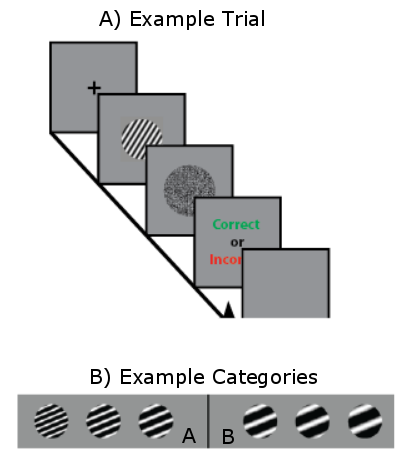
\includegraphics[width=.5\textwidth]{../figures/fig_design_exp_1.png}
  \caption{
      Example trial and category problem. A) Events that
      occurred on each trial. B) An example of a typical
      category structure.
}
  \label{fig:trial}
\end{figure}

\begin{table}
    \caption{
        Durations (in s) of Trial Events in each Condition.
    }
    \label{conditions_exp_1}
    \begin{tabular}{c|cccc}
        Conditions & Stim & Mask & FB & ITI \\[0.5ex] \hline Control & RT & 0.5 &
        1.0 & 0.5 \\[0.5ex]
        \\[-1.5ex] Delayed Feedback &
        RT & 3.5 & 1.0 & 0.5 \\[0.5ex]   Long ITI & RT & 0.5 & 1.0 & 3.5
        \\[0.5ex]
    \end{tabular}
\end{table}

\subsubsection{Participants}
Fifty-nine participants participated in Experiment 1. All
were UCSB undergraduates and received course credit for
their participation. All had normal or corrected to normal
vision. We randomly assigned each participant to one of
three conditions (target $N>16$ per condition based on
similar previous research): Delayed Feedback ($N = 20$);
Long ITI ($N = 21$), Control ($ N = 17$). All participants
gave written informed consent before participating in the
study. All experimental protocols were approved by the
University of California at Santa Barbara Human Subjects
Committee in the Office of Research Development and
Administration.

\subsection{Results}
Figure \ref{fig_mm_hist_1} shows a relative frequency
histogram of the trials-to-criterion observed across all
three conditions. The histogram shows that the majority of
participants were able to learn each problem on average in
less than 100 trials. However, this histogram also shows
that a subset of participants required many more trials to
learn each problem. Given that each problem is very simple
and that the relevant dimension of each problem is
explicitly instructed to participants, it is likely that the
participants in the tails of this distribution did not pay
attention to the instructions, were not motivated to learn
the task, were distracted by other factors, or should be
considered outliers for some other reason. 

\begin{figure}
  \centering
  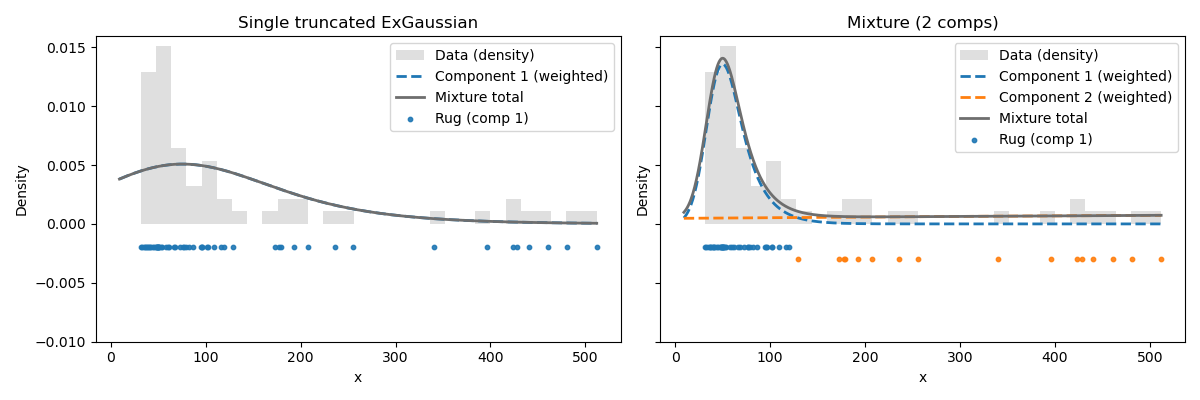
\includegraphics[width=.8\textwidth]{../figures/fig_exp_1_mm_trunc_exgauss_compare.png}
  \caption{
      Relative frequency histogram of the
      trials-to-criterion observed across all three
      conditions in Experiment 1 and the fit of a single
      Exponential-Gaussian distribution (Left) and a
      two-component Exponential-Gaussian mixture model
      (Right). In the right panel, the blue dashed line is
      the first higher performance component, the orange
      dashed line is the second lower performance component.
      The gray solid line is the sum of the two components.
      Rug plots along the x-axes show the individual data
      colored by their assignment to either the higher or
      lower performance component.  The two-component model
      provided a significantly better fit according to AIC,
      BIC, and a likelihood ratio test.
}
  \label{fig_mm_hist_1}
\end{figure}

We modeled the distribution shown in Figure
\ref{fig_mm_hist_1} using a mixture of Exponential-Gaussian
distributions with two components, each truncated to the
range of possible trials-to-criterion values (i.e., $[9,
512]$). The first component captured participants with a
relatively low mean number of trials-to-criterion, while the
second component identified outliers according to the above
rationale.  We estimated this model via MLE with proper
normalization on the tasks bounded support and compared them
via AIC, BIC, and a parametric bootstrap likelihood-ratio
test (LRT).  We compared the MLE fit of this two-component
model to a single-component Exponential-Gaussian model using
the Akaike Information Criterion (AIC) and Bayesian
Information Criterion (BIC), both of which indicated a
better fit for the two-component model 
(
$\mathrm{AIC}_1=692.15$ vs. $\mathrm{AIC}_2=652.81$; 
$\mathrm{BIC}_1=698.33$ vs. $\mathrm{BIC}_2=667.23$
)
Additionally, a bootstrap likelihood ratio test confirmed
that the two-component model provided a significantly better
fit than the one-component model ($D=42.84$,
$p_{\text{boot}}\approx 0.0099$) Participants that were
deemed to most likely to belong in the low-performance
Gaussian by this analysis were excluded from further
analysis. After making these exlcusions, we were left with
the following sample sizes:  Control condition ($ N = 11$);
Delayed-Feedback condition ($N = 14$); Long-ITI condition
($N = 17$).

Figure \ref{fig_exp_1_t2c}A shows the mean
trials-to-criterion in each condition of Experiment 1.  A
one-way ANOVA revealed a significant effect of condition
($F(2, 39) = 6.17$, $p < .01$, $\eta^2 = .24$) and planned
comparisons revealed that performance in the
Delayed-Feedback condition was significantly worse than in
either the Control condition ($t(23.00) = 2.70$, $p < .05$)
or the Long-ITI condition ($t(20.96) = 2.94$, $p < .01$).
Performance in the Control and Long-ITI conditions did not
differ significantly from each other ($t(17.99) = 0.22$, $p
= .83$).

Figure \ref{fig_exp_1_t2c}B shows the mean number of
problems solved in each condition of Experiment 1. A one-way
ANOVA revealed a significant effect of condition ($F(2, 39)
= 5.77$, $p < .01$, $\eta^2 = .23$). Planned comparisons
revealed that performance in the Delayed-Feedback condition
was significantly worse than in the Control condition
($t(18.54) = -3.28$, $p < .01$) and worse than in the Long
ITI condition ($t(21.60) = -2.14$, $p < .05$).  Performance
in the Control and Long-ITI conditions did not differ
significantly from each other ($t(25.97) = -1.50$, $p=.15$).

\begin{figure}
  \centering
  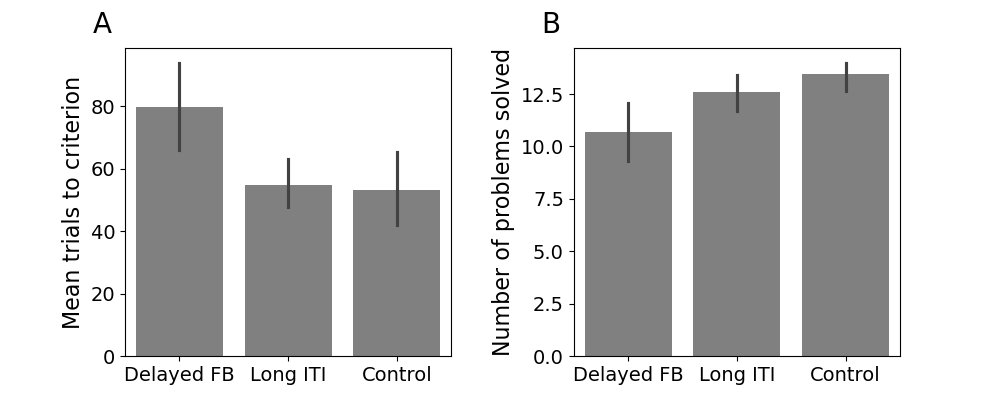
\includegraphics[width=.8\textwidth]{../figures/fig_exp_1_t2c.png}
    \caption{
        \textbf{A}: Mean trials to criterion in each
        condition of Experiment 1. Error bars are standard
        errors of the mean.
        %
        \textbf{B}: Mean number of problems solved in each
        condition of Experiment 1. Error bars are standard
        errors of the mean.
}
  \label{fig_exp_1_t2c}
\end{figure}

\section{Experiment 2}
Experiment 2 was designed to reinforce the findings of
Experiment 1 by using the same design but with stimuli that
have binary-valued dimensions, thereby eliminating criterial
learning. Unlike Experiment 1, we did not explicitly
instruct participants on the relevant stimulus dimension in
Experiment 2.  While Experiment 1 isolated criterial
learning from rule selection and rule switching, this
experiment isolates rule selection and switching from
criterial learning. Therefore, Experiment 2 was designed to
test whether the impaired learning that we observed in
Experiment 1 when the feedback was delayed can be attributed
principally to criterial learning or whether it could be due
to some more general category-learning process.

\subsection{Method}

\subsubsection{Apparatus}
The apparatus was the same as in Experiment 1.

\subsubsection{Stimuli and Categories}
The stimuli consisted of colored geometric figures presented
on a colored background. These varied across six binary
dimensions: the number of items (either one or two), the
size of the items (small or large), the color of the items
(yellow or blue), the shape of the items (circle or square),
the texture of the background (smooth or rough), and the
orientation of the background (horizontal or tilted by 20
degrees). This combination resulted in a total of 64 unique
stimuli ($2^6$). An example trial and stimuli are shown in
Figure \ref{fig_design_exp_2}. In all conditions, the order
of stimulus presentation was fully randomized for each
participant, and the relevant dimension for each problem was
selected randomly without replacement from the set of six
dimensions.

\begin{figure}
  \centering
  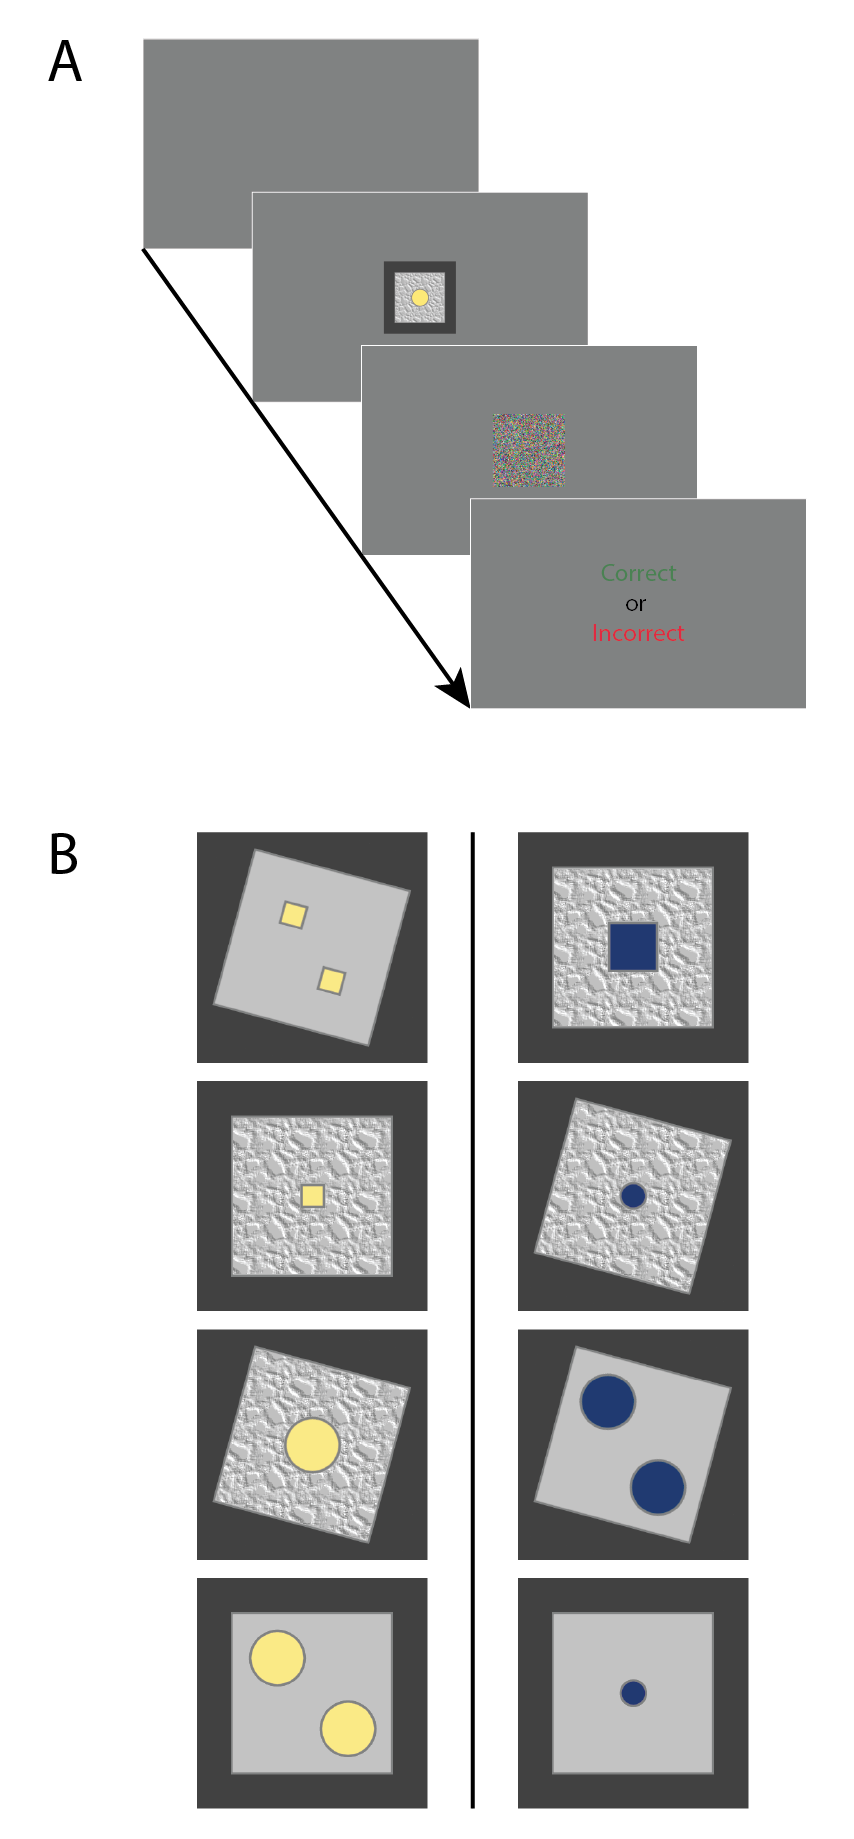
\includegraphics[width=.5\textwidth]{../figures/fig_design_exp_2.png}
  \caption{
      \textbf{A:} An example trial from Experiment 2.
      \textbf{B:} Eight example stimuli (out of 64 total
      stimuli) from a possible one-dimensional rule problem.
      In this case the correct rule is `A' if the shape
      color is yellow and `B' if the shape color is blue.
      The solid line represents the category boundary.
}
  \label{fig_design_exp_2}
\end{figure}

\subsubsection{Procedure}
Participants received detailed instructions about the task.
However, unlike in Experiment 1, they were not informed of
the relevant dimension or the correct rule. The trial timing
for the Delayed-Feedback and Long-ITI conditions in
Experiment 2 were the same as in Experiment 1. Experiment 2
did not include a condition that was analogous to the
Control condition of Experiment 1. Participants practiced
each problem until they responded correctly on 12
consecutive trials. At this point, the problem changed. Each
participant completed as many problems as possible in 600
trials or until they had been in the lab for 30 minutes
(including time to acquire consent and give instructions),
at which point the session was terminated.

\subsubsection{Participants}
Thirty-four participants participated in Experiment 2. All
were Macquarie University undergraduates and received course
credit for their participation. All had normal or corrected
to normal vision. We randomly assigned each participant to
one of two conditions: Delayed Feedback ($N = 17$) or Long
ITI ($N = 17$).  All participants gave written informed
consent before participating in the study. All experimental
protocols were approved by the Macquarie University Human
Research Ethics Committee (protocol number: 52020339922086). 

\subsection{Results}
Figure \ref{fig_mm_hist_2} shows a relative frequency
histogram of the trials-to-criterion observed in both
conditions. The histogram shows that the majority of
participants were able to learn each problem on average in
less than 100 trials.  Unlike Experiment 1, there were no
highly suspicious outliers in this data set. Nevertheless,
for symmetry with Experiment 1, we performed the same
Gaussian mixture model analysis as used there. The
two-component model provided a slightly smaller AIC value
(324.75 vs. 317.18), and a slightly larger BIC value (329.33
vs. 327.87). The bootstrap likelihood-ratio test was not
significant ($D = 11.41, p_{\text{boot}} \approx 0.2277$).
We therefore did not exclude any participants from further
analysis in Experiment 1.

\begin{figure}
  \centering
  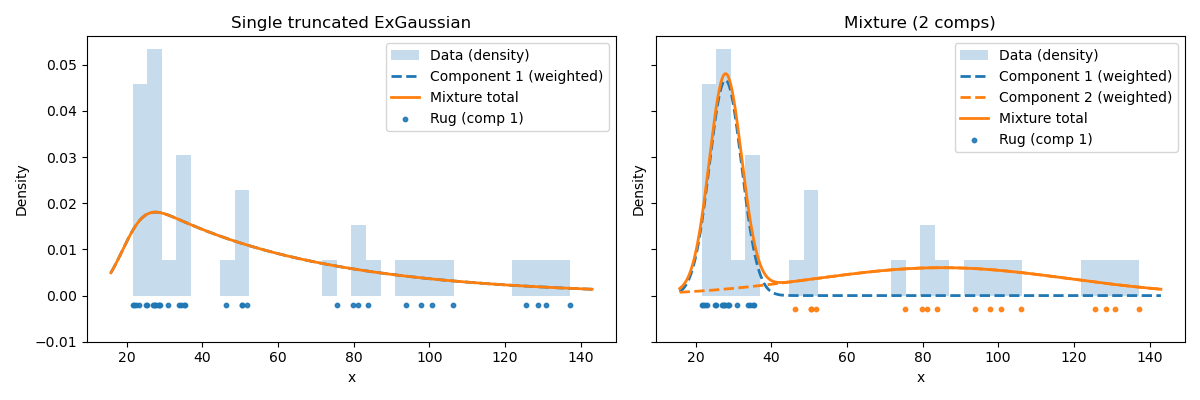
\includegraphics[width=.8\textwidth]{../figures/fig_exp_2_mm_trunc_exgauss_compare.png}
  \caption{
      Relative frequency histogram of the
      trials-to-criterion observed across all three
      conditions in Experiment 2. The black line represents
      the best fit of the one-component Gaussian Mixture
      Model, and the red line represents the best fit of the
      two-component Gaussian Mixture Model.
}
  \label{fig_mm_hist_2}
\end{figure}

Figure \ref{fig_exp_2_t2c}A shows the mean
trials-to-criterion in each condition of Experiment 2. An
independent-samples t-test revealed no significant effect of
condition ($t(32.0)=0.69$, $p = .50$, $\eta^2 = .01$).  The
mean number of problems solved by each participant is shown
in Figure \ref{fig_exp_2_t2c}B. An independent-samples
t-test revealed no significant effect of condition ($t(32) =
-0.49$, $p = .63$, $\eta^2 = .01$).

\begin{figure}
  \centering
  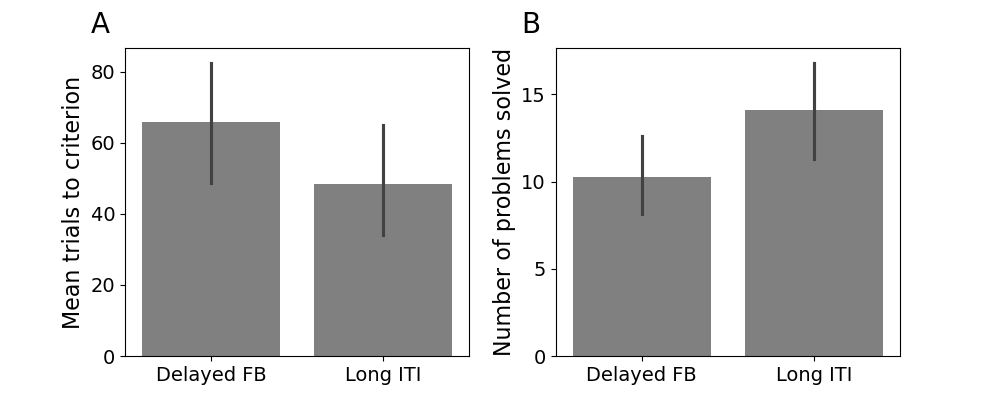
\includegraphics[width=.8\textwidth]{../figures/fig_exp_2_t2c.png}
    \caption{
        \textbf{A}: Mean trials to criterion in each
        condition of Experiment 2. Error bars are standard
        errors of the mean.
        %
        \textbf{B}: Mean number of problems solved in each
        condition of Experiment 2. Error bars are standard
        errors of the mean.
}
  \label{fig_exp_2_t2c}
\end{figure}

\subsection{Discussion of Experiments 1 and 2}
Experiment 1 clearly showed that a short feedback delay of
3.5 s slowed criterial learning. In contrast, increasing the
ITI to this same value had no effect on learning. The task
we used was one-dimensional category learning, but we
isolated criterial learning by instructing participants
about the optimal strategy. Specifically, we told them which
stimulus dimension was relevant and that there was no
trial-by-trial variability on the irrelevant dimension.
Although these results strongly suggest that the feedback
delay had its interfering effects on criterial learning,
Experiment 2 was designed to confirm this inference. The
goal here was to examine the effects of the same feedback
delays and ITIs on performance in a one-dimensional
category-learning task that did not require any criterial
learning, but did require category-learning processes that
are thought to mediate rule discovery (e.g., rule selection
and switching). If the feedback delay effects observed in
Experiment 1 were acting on some general category-learning
skill then we should have seen the same interfering effects
of feedback delay in Experiment 2. However, if the
feedback-delay interference of Experiment 1 was operating
selectively on criterial learning, then it should disappear
in Experiment 2, since no criterial learning was required.
Our results strongly supported this latter prediction.
Therefore, Experiments 2 and 3 together strongly suggest
that criterial learning is impaired by feedback delays and
is relatively unaffected by the length of the ITI.

Two prior studies investigated similar issues. First, Ell
and colleagues reported that feedback delay and also a
concurrent memory-scanning task each impaired rule-based
category learning \parencite{ell2009critrial}. Based on
these results, they hypothesized that criterial learning may
be tied to working-memory capacity and therefore to explicit
cognitive mechanisms. However, criterial learning was
confounded with rule selection and task difficulty in their
design.  Furthermore, \textcite{ell2009critrial} found that
feedback delay only impaired learning when working memory
demand was high -- that is, when participants had to learn
more than one response criterion for optimal performance. In
contrast, we found that feedback delay impairs learning even
when working memory demands are trivial (participants never
have to keep in mind more than one criterion).

Second, \textcite{bohil2014implicit} reported that the
effects of unequal base rates on criterion placement in
rule-based category learning were diminished under delayed
feedback and also under an observational training protocol
that is also thought to selectively impair basal
ganglia-dependent associative-learning mechanisms. These
results are consistent with our findings. However, because
they were obtained by manipulating base rates, it is
difficult to conclude that the delay affected criterial
learning, \emph{per se}. For example, consider a simple
two-stage model in which the first stage learns the base
rates and the second stage uses what the first stage learned
to adjust the response criterion appropriately. The
\textcite{bohil2014implicit} results are also consistent
with the hypothesis that the feedback delay impaired the
first of these stages but not the second. Our results
strongly suggest that feedback delays impair criterial
learning (and therefore the second of these hypothetical
stages).

\section{General Discussion}
We developed novel models of criterial learning that were
designed to explore how feedback delay and ITI duration
affect criterial learning.  One class of model assumed that
decisions are made by comparing the current percept to a
stored referent, or criterion, and that the remembered value
of this criterion is updated following error feedback via a
gradient-descent learning rule.  This class of model
generates sensitivity to feedback delay and ITI duration
through (1) directly assuming that the update rule is
inversely scaled by the feedback delay, (2) assuming that
the representation of the percept drifts over time, or (3)
assuming the representation of the criterion drifts over
time.  Simulations of these models in a task that was
structurally identical to Experiment 1 revealed that this
class of model typically predicts that feedback delay in
more impairing than a long ITI only when the update rule is
explicitly delay-sensitive.  Otherwise, it typically
predicts that long ITIs are more impairing than feedback
delays.

The second model class, reinforcement-learning models,
assumes that criterial learning arises through the gradual
formation of stimulus-response associations, rather than via
the construction of a response criterion.  These models can
generate sensitivity to feedback delay and ITI duration
through the same two mechanisms as the first class of
models. However, since these models do not explicitly
represent a criterion, they do not assume that the
representation of the criterion drifts over time.   This
class of model  typically predicts that feedback delay is
more impairing than a long ITI across wide ranges of
parameter values.

The experiments were designed to test these predictions. Our
results strongly suggested that human criterial learning is
sensitive to feedback delay but not to the ITI duration.
These results shed important constraints on the new models
of criterial learning developed here. In particular, the
reinforcement-learning models are consistent with the
observed behavioural data across wide ranges of their
parameter spaces, regardless of whether or not the update
rule is delay-sensitive.  However, the models that assume a
stored criterion are also consistent with the observed
behavioral data, but only when the update rule is
delay-sensitive.

One natural neural underpinning for models that assume a
stored criterion is that the criterion is maintained in
working memory. However, since it is widely accepted that
working memory is largely insensitive to both feedback delay
and ITI duration, this interpretation is difficult to
reconcile with our results suggesting a delay-sensitive
update rule is required for this class of model. An
alternative possibility for where the criterion might be
encoded in a more stable memory system.  One appealing
candidate for this function is the cerebellum, where
synaptic plasticity has been shown to follow a gradient
descent learning rule and also to be sensitive to feedback
timing \parencite{brudner2016delayed, held_adaptation_1966,
honda_adaptation_2012, kitazawa_effects_1995,
kitazawa_prism_2002}.   Finally, the reinforcement-learning
model draws on the idea that criterial learning could emerge
through stimulus-response association learning driven by
dopamine-dependent synaptic plasticity in the striatum. This
process aligns with established theories of category
learning that posit a key role to this learning process in
the basal ganglia \cite{AshbyCOVIS1998}.

Our results do not strongly favor one model over another.
The critical disagreement between these accounts is whether
the criterion has any real psychological meaning. One class
assumes the criterion is stored in memory and compared
against incoming stimuli to generate responses.  The
reinforcement-learning model, in contrast, makes very
different psychological assumptions. This model assumes that
behaviors described as ``criterial learning'' are actually
mediated by the learning of stimulus-response associations.
According to this account, the criterion has no internal
representation and therefore no psychological meaning.
Testing between these two very different accounts of
criterial learning should be a focus of future research. 

We are not aware of any data that directly addresses the
question of whether a response criterion is a fundamental
psychological construct, or whether it is unnecessary. Even
so, there are some results in the category-learning
literature that support the interpretation of the
reinforcement-learning model. In information-integration
(II) category-learning tasks, the optimal strategy is
similarity-based, and difficult or impossible to describe
verbally \parencite[e.g.,][]{AshbyValentin2018}. When the
stimuli vary on two dimensions, the stimuli from contrasting
categories can be partitioned by a decision bound that is
conceptually similar to a response criterion. In both cases,
all stimuli on one side are associated with one response,
and all stimuli on the other side are associated with the
contrasting response. Furthermore, in agreement with
Experiment 1, II category learning is impaired by short
feedback delays \parencite{MaddoxAshbyBohil2003,
MaddoxIng2005}. The analogous question in II category
learning is whether the decision bound is learned directly
or whether it is simply the set of points that divide the
perceptual space into contrasting response regions.  In
fact, the evidence strongly supports this latter
interpretation \parencite{AshbyWaldron1999, CasaleEtAl2012}.
For example, if the decision bound is learned, then it
should be possible to apply this bound to novel stimuli.
With rule-based categories, this is easy for participants,
but with II categories there is no evidence that the
response strategy that participants learn can be generalized
to novel stimuli \parencite{CasaleEtAl2012} -- a result that
strongly supports the hypothesis that the decision bound has
no psychological meaning. 

Our results clearly demonstrate that criterial learning is
impaired by delayed feedback, and not by extending the
intertrial interval. These results are consistent with the
hypothesis that criterial learning is a form of
basal-ganglia mediated associative learning, and are
inconsistent with hypotheses that criterial learning is a
working-memory-based process. Thus, our results provide a
critical constraint on future models of rule-based
classification and decision making, and possibly also on
more general accounts of criterion setting, such as in
signal detection theory.

Previous studies have failed to find that feedback delays
impair rule-based category learning, and on the face of it,
this seems to contradict our finding that feedback delays
impair criterial learning. However, all earlier RB studies
that looked for effects of a feedback delay, either used
binary-valued stimulus dimension and so no criterial
learning was needed, or else set the response criterion
exactly midway between the category prototypes, which makes
criterial learning trivial. For example, under these
conditions, criterial learning might not even require
feedback. The unsupervised category-learning experiments
reported by \textcite{ashby1999dominance} provide strong
support for this because all of their rule-based
participants learned the correct criterion (which was midway
between the category means), even though the task was
completely unsupervised. Moreover, all previous studies
failed to isolate criterial learning, so even if there was
an effect of feedback delay on criterial learning, it could
have been masked by larger effects caused by other
rule-learning processes.

Criterial learning is among the most classic and ubiquitous
of all cognitive skills. For example, signal-detection
theory teaches that it is the central form of learning in an
enormous range of decision-making tasks -- everything from
simple YES-NO detection of a weak signal to assessing the
guilt or innocence of a defendant in a jury trial. Our
results suggest that even in simple rule-based tasks,
criterial learning seems to be subserved, at least in part,
by associative mechanisms. Most current theories tend to
classify tasks as either executive function (e.g.,
rule-based category learning) or procedural (e.g., mirror
tracing). Our results suggest that such classification
schemes might oversimplify how humans perform these tasks,
and therefore that much more work is needed to understand
how different learning and memory systems interact.

\section{Transparency and Openness}
All data have been made publicly available in the following
GitHub repository:
\url{https://github.com/crossley/crit_learn_delay}

\section{Author Notes}
Preparation of this article was supported by Public Health
Service Grant MH2R01-063760.

\printbibliography

\end{document}
